\documentclass[conference]{IEEEtran}
\IEEEoverridecommandlockouts
% The preceding line is only needed to identify funding in the first footnote. If that is unneeded, please comment it out.

% ============================================
% PACKAGES
% ============================================
\usepackage{cite}
\usepackage{amsmath,amssymb,amsfonts}
\usepackage{algorithmic}
\usepackage{graphicx}
\usepackage{textcomp}
\usepackage{xcolor}
\usepackage{booktabs}
\usepackage{hyperref}
\usepackage{enumitem}
\usepackage{tikz}
\usetikzlibrary{shapes.geometric, arrows.meta, positioning, calc}

\def\BibTeX{{\rm B\kern-.05em{\sc i\kern-.025em b}\kern-.08em
    T\kern-.1667em\lower.7ex\hbox{E}\kern-.125emX}}

% ============================================
% DOCUMENT
% ============================================
\begin{document}

\title{Vulnerabilities of Small Language Models: A Systematic Literature Review}

\author{\IEEEauthorblockN{Daniel Dias}
\IEEEauthorblockA{\textit{Department of Informatics Engineering} \\
\textit{Polytechnic School of Porto}\\
Porto, Portugal \\
1240145@isep.ipp.pt}
}

\maketitle

% ============================================
% ABSTRACT
% ============================================
\begin{abstract}
\textbf{Context:} Small Language Models (SLMs), typically defined as models with fewer than 7 billion parameters, have emerged as efficient alternatives to Large Language Models (LLMs) for deployment in resource-constrained environments such as edge devices, mobile applications, and IoT systems. As their adoption accelerates, understanding their security vulnerabilities becomes critical.
\textbf{Goal:} This systematic literature review aims to identify, categorize, and analyze the security vulnerabilities specific to small language models, examining how these vulnerabilities differ from those observed in larger models and evaluating proposed mitigation strategies.
\textbf{Method:} We conducted a systematic literature review following PRISMA guidelines, searching multiple databases including IEEE Xplore, ACM Digital Library, arXiv, and Semantic Scholar. Studies were selected based on predefined inclusion and exclusion criteria, with quality assessment performed using established protocols.
\textbf{Results:} Our analysis reveals that SLMs exhibit distinct vulnerability profiles compared to their larger counterparts, with particular susceptibility to prompt injection, jailbreaking, and adversarial attacks. The reduced parameter count often limits the implementation of safety mechanisms, creating unique security challenges.
\textbf{Conclusion:} This review provides the first comprehensive taxonomy of SLM-specific vulnerabilities and identifies critical gaps in current research, offering a foundation for future security research in small language models.
\end{abstract}

\begin{IEEEkeywords}
Small Language Models, Security Vulnerabilities, Prompt Injection, Jailbreaking, Adversarial Attacks, Systematic Literature Review
\end{IEEEkeywords}

% ============================================
% I. INTRODUCTION
% ============================================
\section{Introduction}

The field of natural language processing has undergone a fundamental transformation with the advent of transformer-based architectures \cite{vaswani2017attention} and the subsequent development of Large Language Models. Systems such as GPT \cite{achiam2024gpt4}, Claude, and Gemini have demonstrated remarkable capabilities in reasoning, code generation, and creative tasks, driven by scaling to hundreds of billions of parameters \cite{brown2020language,zhao2023survey}. These foundation models have reshaped expectations for artificial intelligence and attracted substantial industrial investment \cite{bommasani2021opportunities}.

Yet a critical countertrend is emerging: the rise of small language models designed for practical deployment and mitigating private data leakage. Small language models, typically defined as transformer-based architectures with around 7-10 billion parameters \cite{lu2024slm_survey, belcak2025slm_agentic}, have emerged as compelling alternatives that address fundamental limitations of their larger counterparts. SLMs require substantially less memory and processing power, enabling deployment on hardware ranging from consumer GPUs to mobile devices and IoT systems, with proportionally reduced operational costs \cite{lu2024slm_survey, tang2025demystifying}. Edge deployment enables real-time inference without network latency, critical for autonomous systems, industrial automation, and responsive interfaces. Privacy-sensitive applications benefit from local inference, eliminating the need to transmit confidential data to cloud services. Models such as Microsoft's Phi-2 \cite{phi2}, TinyLlama \cite{tinyllama}, and Google's Gemma \cite{gemma} have demonstrated that compact architectures can achieve remarkable performance on targeted tasks, challenging assumptions about the necessity of scale. Recent work from NVIDIA researchers argues that small language models represent the future of agentic AI systems, as the specialized and repetitive tasks characteristic of such systems are better suited to smaller, more efficient models \cite{belcak2025slm_agentic}. This perspective reflects a broader recognition that practical considerations of cost, latency, and deployment constraints increasingly favor compact alternatives.

However, the rapid adoption of small language models has outpaced systematic investigation of their security properties, creating significant risks for deploying organizations. Zhang et al. found that nearly half of the 63 SLMs they tested exhibited attack success rates exceeding 40\% against jailbreak attempts, while over one-third failed to resist even straightforward harmful requests \cite{zhang2025slm_jailbreak}. The fundamental challenge lies in the tension between model capacity and security implementation: safety mechanisms that function effectively in models with hundreds of billions of parameters may degrade or fail entirely when compressed into smaller architectures \cite{li2025quantized_jailbreak}. Yi et al. documented how compression techniques commonly used to create deployable SLMs can compromise security robustness, revealing ``submerged threats'' that emerge from efficiency optimizations \cite{yi2025slm_submerged}. Edge deployment introduces additional attack surfaces, as models operating in physically accessible environments face threats ranging from adversarial input injection \cite{wang2022adversarial_nlp_survey} to direct model extraction \cite{carlini2024stealing,yao2024survey_extraction}. The combination of reduced defensive capacity and expanded attack surface creates a security landscape that demands dedicated investigation, distinct from the extensive but LLM-focused security literature \cite{xu2024jailbreak_survey}.

% ============================================
% II. METHODOLOGY
% ============================================
\section{Methodology}

This systematic literature review follows the Preferred Reporting Items for Systematic Reviews and Meta-Analyses (PRISMA) 2020 guidelines \cite{page2021prisma} and adopts established protocols for conducting systematic reviews in software engineering \cite{kitchenham2009systematic}. The methodology encompasses research question formulation, systematic search strategy development, study selection through predefined criteria, and thematic data synthesis.

\subsection{Research Questions}

To address the main research question---\textit{What is the current state of knowledge regarding security vulnerabilities in Small Language Models, and how do these vulnerabilities manifest differently compared to Large Language Models?}---the most relevant and recent literature will be analyzed according to four sub-questions (see Table~\ref{tab:research_questions}).

\begin{table}[htbp]
\caption{Research Questions}
\label{tab:research_questions}
\renewcommand{\arraystretch}{1.4}
\begin{center}
\begin{tabular}{|c|p{6.5cm}|}
\hline
\textbf{RQ} & \textbf{Description} \\
\hline
RQ1 & What types of security vulnerabilities have been identified in Small Language Models, and how are they characterized and categorized in the existing literature? \\
\hline
RQ2 & How do vulnerabilities in SLMs differ from those in LLMs in terms of attack success rates, exploitability, and severity? \\
\hline
RQ3 & What specific architectural or deployment characteristics of SLMs contribute to their unique vulnerability profiles? \\
\hline
RQ4 & What mitigation strategies and defense mechanisms have been proposed for SLM vulnerabilities, and what empirical evidence supports their effectiveness? \\
\hline
\end{tabular}
\end{center}
\end{table}

\vspace{0.5em}

The \textbf{first sub-question} focuses on identifying the types of security vulnerabilities that have been documented in small language models. This analysis will provide insight into current attack taxonomies, including jailbreaking, prompt injection, backdoor attacks, adversarial examples, membership inference, and model extraction attacks targeting SLMs.

The \textbf{second sub-question} aims to explore the comparative security landscape between small and large language models. This is crucial for understanding whether the reduced parameter count of SLMs correlates with increased susceptibility to attacks, and how attack success rates vary across model scales.

The \textbf{third sub-question} investigates the root causes of SLM-specific vulnerabilities, examining how architectural decisions such as compression, quantization, and knowledge distillation affect security properties. Additionally, this includes evaluating how edge deployment constraints and resource limitations impact the implementation of safety mechanisms.

Finally, the \textbf{fourth sub-question} focuses on identifying the defense mechanisms and mitigation strategies proposed in the literature for protecting SLMs. This includes evaluating both theoretical proposals and empirically validated countermeasures, assessing their effectiveness across different vulnerability categories.

\subsection{Search Strategy}

The search strategy employed in this review was designed to identify the most relevant and up-to-date studies available in the scientific literature related to the research topic. The process was structured into three main stages:

\begin{enumerate}[noitemsep]
    \item \textbf{Definition of search sources:} selection of recognized academic databases and scientific repositories to ensure comprehensive coverage of relevant publications.
    \item \textbf{Definition of search terms:} inclusion of keywords and logical combinations that accurately reflect the core concepts of the study, such as ``small language model'', ``vulnerability'', ``jailbreak'', and ``adversarial attack''.
    \item \textbf{Study selection and data extraction:} application of inclusion and exclusion criteria to guarantee the relevance, quality, and methodological rigor of the analyzed works.
\end{enumerate}

This structured approach ensures that the review process remains transparent, replicable, and focused on collecting the most significant contributions to the research question.

\subsubsection{Definition of Search Sources}

The first step of the search strategy was to identify and define which sources would be considered while conducting the SLR. For this study, searches were carried out in several major electronic databases (see Table~\ref{tab:databases}). These databases were selected due to their broad coverage of peer-reviewed journal articles, conference proceedings, and preprints in the fields of computer science, artificial intelligence, natural language processing, and cybersecurity, which are directly relevant to the topic of small language model vulnerabilities.

\begin{table}[htbp]
\caption{Electronic Databases}
\label{tab:databases}
\renewcommand{\arraystretch}{1.3}
\begin{center}
\begin{tabular}{|c|l|l|}
\hline
\textbf{ID} & \textbf{Database} & \textbf{URL} \\
\hline
ED1 & arXiv & \url{https://arxiv.org/} \\
ED2 & Semantic Scholar & \url{https://semanticscholar.org/} \\
ED3 & ACL Anthology & \url{https://aclanthology.org/} \\
ED4 & IEEE Xplore & \url{https://ieeexplore.ieee.org/} \\
ED5 & ACM Digital Library & \url{https://dl.acm.org/} \\
\hline
\end{tabular}
\end{center}
\end{table}

Additionally, gray literature sources including technical reports from NVIDIA Research, Microsoft Security, and Anthropic were consulted to capture emerging findings not yet published in peer-reviewed venues.

\vspace{0.5em}

\subsubsection{Definition of Search Terms}

The second step of the search strategy involved defining a set of search strings that accurately reflected the research questions formulated for this study. The terms were derived from the main concepts present in the research scope: small language models, security vulnerabilities, and attack/defense mechanisms. Boolean operators and synonyms were used to broaden the search and ensure coverage across different scientific databases.

\vspace{0.5em}

Table~\ref{tab:model_terms} presents the search terms used to identify studies related to small language models, including both generic descriptors and specific model architectures.

\begin{table}[htbp]
\caption{Search Terms: Model Identification}
\label{tab:model_terms}
\renewcommand{\arraystretch}{1.3}
\begin{center}
\begin{tabular}{|l|p{5.8cm}|}
\hline
\textbf{Category} & \textbf{Search Terms} \\
\hline
Generic SLM Terms & ``small language model'' OR ``SLM'' OR ``lightweight language model'' OR ``edge language model'' OR ``compact language model'' OR ``efficient language model'' \\
\hline
Decoder-only Models & ``Phi-2'' OR ``Phi-3'' OR ``Gemma'' OR ``TinyLlama'' OR ``Llama 7B'' OR ``Mistral 7B'' OR ``Qwen'' \\
\hline
Encoder-only Models & ``MobileBERT'' OR ``DistilBERT'' OR ``MiniLM'' OR ``ALBERT'' OR ``TinyBERT'' \\
\hline
\end{tabular}
\end{center}
\end{table}

\vspace{0.5em}

Table~\ref{tab:security_terms} presents the search terms used to capture security vulnerabilities and attack types relevant to language models.

\begin{table}[htbp]
\caption{Search Terms: Security and Vulnerabilities}
\label{tab:security_terms}
\renewcommand{\arraystretch}{1.3}
\begin{center}
\begin{tabular}{|l|p{5.8cm}|}
\hline
\textbf{Category} & \textbf{Search Terms} \\
\hline
General Security & ``vulnerability'' OR ``attack'' OR ``security'' OR ``robustness'' OR ``adversarial'' \\
\hline
Prompt-based Attacks & ``jailbreak'' OR ``prompt injection'' OR ``prompt leaking'' OR ``guardrail bypass'' \\
\hline
Training-time Attacks & ``backdoor'' OR ``poisoning'' OR ``data poisoning'' OR ``trojan'' \\
\hline
Privacy Attacks & ``membership inference'' OR ``data extraction'' OR ``model stealing'' OR ``model extraction'' \\
\hline
\end{tabular}
\end{center}
\end{table}

\vspace{0.5em}

The search strings were defined to cover four main pillars of the research scope:

\begin{itemize}
    \item \textbf{Generic SLM Terms:} to capture studies on compact transformer architectures using general terminology such as ``small language model'' or ``lightweight language model''.

    \item \textbf{Specific Model Architectures:} focused on identifying studies related to specific models commonly deployed in resource-constrained environments, distinguishing between encoder-only architectures (BERT variants) and decoder-only architectures (Phi, Gemma, TinyLlama, Llama 7B).

    \item \textbf{General Security and Prompt-based Attacks:} intended to include studies addressing security weaknesses and inference-time attack vectors, such as jailbreaking and prompt injection.

    \item \textbf{Training-time and Privacy Attacks:} to capture studies on attacks that occur during model training (backdoors, poisoning) or that compromise data privacy (membership inference, model extraction).
\end{itemize}

\vspace{0.5em}

The final search query combined these categories using Boolean operators as follows:

\begin{quote}
\small
(Generic SLM Terms \textbf{OR} Decoder-only Models \textbf{OR} Encoder-only Models) \textbf{AND} (General Security \textbf{OR} Prompt-based Attacks \textbf{OR} Training-time Attacks \textbf{OR} Privacy Attacks)
\end{quote}

Date filtering was restricted to publications from January 2020 to December 2025.

\subsection{Inclusion and Exclusion Criteria}

Studies were selected based on the following predefined criteria, which were established prior to conducting the search to ensure objectivity and reproducibility.

\vspace{0.5em}

\textbf{Inclusion Criteria:}
\begin{itemize}
    \item Published between January 2020 and December 2025
    \item Focuses on Small Language Models defined as models with fewer than 10 billion parameters, following the NVIDIA definition \cite{belcak2025slm_agentic}
    \item Addresses security vulnerabilities, attacks, adversarial robustness, or defense mechanisms
    \item Peer-reviewed publication or high-quality preprint with substantial methodology
    \item Published in English
\end{itemize}

\vspace{0.3em}

\textbf{Exclusion Criteria:}
\begin{itemize}
    \item Focuses exclusively on large models ($>$10B parameters) without demonstrated applicability to SLMs
    \item Contains no security or vulnerability component
    \item Non-English publication
    \item Duplicate publication of the same study
    \item Full text not accessible
    \item Workshop papers or extended abstracts without sufficient methodological detail
\end{itemize}

\subsection{Study Selection Process}

The study selection followed a three-stage screening process consistent with PRISMA guidelines. In the first stage, titles of all retrieved records were screened against inclusion criteria, removing obviously irrelevant studies. The second stage involved abstract screening, where remaining studies were evaluated based on their abstracts to assess relevance to SLM security. The third stage comprised full-text assessment, where complete papers were reviewed to confirm eligibility and extract detailed information.

\subsection{Data Extraction and Synthesis}

Data extraction was performed using a standardized form capturing: study metadata (authors, year, venue, DOI), model characteristics (architecture, parameter count, quantization level), vulnerability type (jailbreak, prompt injection, backdoor, adversarial, membership inference, model extraction), attack methodology and success rates, defense mechanisms evaluated, and key findings. The extracted data were synthesized thematically, organizing findings by vulnerability categories rather than individual studies, enabling cross-study comparison and identification of consensus findings and research gaps.

\subsection{PRISMA Flow}

Figure~\ref{fig:prisma} illustrates the study selection process following PRISMA 2020 guidelines. The initial database search yielded 72 records distributed across arXiv (n=26), Semantic Scholar (n=43), and ACL Anthology (n=3), with 3 additional records identified through gray literature sources (NVIDIA Research, Microsoft Security, Anthropic), totaling 75 records. After removing 7 duplicates identified through DOI and title matching, 68 unique records underwent title and abstract screening. Of these, 3 were excluded: 2 for publication date outside the specified range (pre-2020), and 1 for out-of-scope focus on using LLMs for security testing rather than vulnerabilities in SLMs. The remaining 65 studies proceeded to full-text eligibility assessment and were included in the final synthesis.

\begin{figure*}[htbp]
\centering
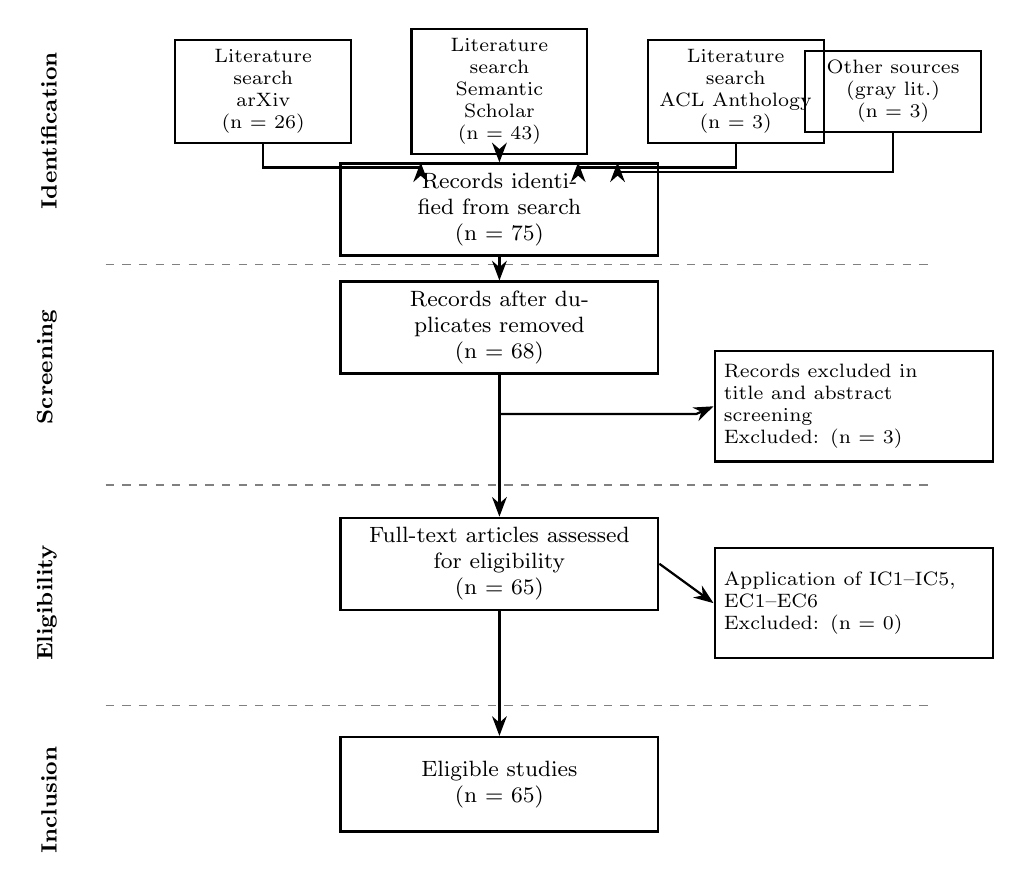
\begin{tikzpicture}[
    % Node styles
    box/.style={rectangle, draw=black, thick, minimum width=2.8cm, minimum height=1.2cm, text centered, text width=2.6cm, font=\footnotesize},
    smallbox/.style={rectangle, draw=black, thick, minimum width=2.2cm, minimum height=1cm, text centered, text width=2cm, font=\scriptsize},
    wideboxaliased/.style={rectangle, draw=black, thick, minimum width=4cm, minimum height=1cm, text centered, text width=3.8cm, font=\footnotesize},
    exclusionbox/.style={rectangle, draw=black, thick, minimum width=3.5cm, minimum height=1.4cm, text centered, text width=3.3cm, font=\scriptsize, align=left},
    stagetext/.style={font=\footnotesize\bfseries, rotate=90, anchor=south},
    arrow/.style={-{Stealth[length=2.5mm]}, thick}
]

% Stage labels (left side)
\node[stagetext] at (-5.5, 0.5) {Identification};
\node[stagetext] at (-5.5, -2.5) {Screening};
\node[stagetext] at (-5.5, -5.5) {Eligibility};
\node[stagetext] at (-5.5, -8) {Inclusion};

% Dashed lines separating stages
\draw[dashed, gray] (-5, -1.2) -- (5.5, -1.2);
\draw[dashed, gray] (-5, -4) -- (5.5, -4);
\draw[dashed, gray] (-5, -6.8) -- (5.5, -6.8);

% IDENTIFICATION STAGE
% Database boxes
\node[smallbox] (arxiv) at (-3, 1) {Literature search\\arXiv\\(n = 26)};
\node[smallbox] (semantic) at (0, 1) {Literature search\\Semantic Scholar\\(n = 43)};
\node[smallbox] (acl) at (3, 1) {Literature search\\ACL Anthology\\(n = 3)};

% Other sources
\node[smallbox] (other) at (5, 1) {Other sources\\(gray lit.)\\(n = 3)};

% Records identified
\node[wideboxaliased] (identified) at (0, -0.5) {Records identified from search\\(n = 75)};

% Arrows from databases to identified
\draw[arrow] (arxiv.south) -- ++(0,-0.3) -| ($(identified.north) + (-1,0)$);
\draw[arrow] (semantic.south) -- ($(identified.north)$);
\draw[arrow] (acl.south) -- ++(0,-0.3) -| ($(identified.north) + (1,0)$);
\draw[arrow] (other.south) -- ++(0,-0.5) -| ($(identified.north) + (1.5,0)$);

% SCREENING STAGE
% Duplicates removed
\node[wideboxaliased] (duplicates) at (0, -2) {Records after duplicates removed\\(n = 68)};

% Excluded at screening
\node[exclusionbox] (excluded1) at (4.5, -3) {Records excluded in\\title and abstract\\screening\\Excluded: (n = 3)};

% Arrows
\draw[arrow] (identified.south) -- (duplicates.north);
\draw[arrow] (duplicates.south) -- ++(0, -0.5) -- ++(2.5, 0) -- (excluded1.west);

% ELIGIBILITY STAGE
% Full-text assessed
\node[wideboxaliased] (fulltext) at (0, -5) {Full-text articles assessed\\for eligibility\\(n = 65)};

% Excluded at full-text
\node[exclusionbox] (excluded2) at (4.5, -5.5) {Application of IC1--IC5,\\EC1--EC6\\Excluded: (n = 0)};

% Arrows
\draw[arrow] (duplicates.south) -- ++(0,-0.3) -- (fulltext.north);
\draw[arrow] (fulltext.east) -- (excluded2.west);

% INCLUSION STAGE
% Final included
\node[wideboxaliased, minimum height=1.2cm] (included) at (0, -7.8) {Eligible studies\\(n = 65)};

% Arrow
\draw[arrow] (fulltext.south) -- (included.north);

\end{tikzpicture}
\caption{PRISMA 2020 flow diagram showing study selection process.}
\label{fig:prisma}
\end{figure*}

% ============================================
% IV. RESULTS
% ============================================
\section{Results}

% Placeholder for results content
This section will present the findings of the systematic review organized by thematic categories.

\subsection{Study Selection}

% Content to be added

\subsection{Vulnerability Categories}

% Content to be added

\subsection{Mitigation Strategies}

% Content to be added

% ============================================
% V. DISCUSSION
% ============================================
\section{Discussion}

% Placeholder for discussion content
This section will interpret the findings and discuss their implications for research and practice.

\subsection{Key Findings}

% Content to be added

\subsection{Implications for Practice}

% Content to be added

\subsection{Limitations}

% Content to be added

% ============================================
% VI. CONCLUSIONS
% ============================================
\section{Conclusions}

% Placeholder for conclusions content
This section will summarize the key contributions and outline future research directions.

% ============================================
% REFERENCES
% ============================================
\bibliographystyle{IEEEtran}
\bibliography{references}

\end{document}
